\documentclass[11pt]{article}
\usepackage[paper=letterpaper,margin=1in]{geometry}

\usepackage[parfill]{parskip}
\usepackage{amsmath}
\usepackage{graphicx}

\begin{document}
\thispagestyle{empty}
\begin{center}
{\large CS 310}\\
Assignment 321
\end{center}

\begin{flushright}
Cameron Moberg
\end{flushright}

There are several ways to solve the closest-pair problem, the two done in this analysis are the brute-force method, where you compare every single pair and find the smallest, and the divide-and-conquer method. The purpose of this study is to perform an empirical analysis of the two methods.

For both methods, the value for $n$ is taken to be the number of points in the plane.

To analyze the brute-force algorithm, we chose calculating the distance on line 67 as the basic operation, because this happens most frequently, is the most expensive, and is the philosophical heart of this algorithm.

An empirical analysis of running the algorithm for multiple values of
$n$ produces the results shown below. Standard function $f(n) = n^2$ with constant multipliers, has been added to
illustrate the analysis.

\begin{center}
    % GNUPLOT: LaTeX picture with Postscript
\begingroup
  \makeatletter
  \providecommand\color[2][]{%
    \GenericError{(gnuplot) \space\space\space\@spaces}{%
      Package color not loaded in conjunction with
      terminal option `colourtext'%
    }{See the gnuplot documentation for explanation.%
    }{Either use 'blacktext' in gnuplot or load the package
      color.sty in LaTeX.}%
    \renewcommand\color[2][]{}%
  }%
  \providecommand\includegraphics[2][]{%
    \GenericError{(gnuplot) \space\space\space\@spaces}{%
      Package graphicx or graphics not loaded%
    }{See the gnuplot documentation for explanation.%
    }{The gnuplot epslatex terminal needs graphicx.sty or graphics.sty.}%
    \renewcommand\includegraphics[2][]{}%
  }%
  \providecommand\rotatebox[2]{#2}%
  \@ifundefined{ifGPcolor}{%
    \newif\ifGPcolor
    \GPcolorfalse
  }{}%
  \@ifundefined{ifGPblacktext}{%
    \newif\ifGPblacktext
    \GPblacktexttrue
  }{}%
  % define a \g@addto@macro without @ in the name:
  \let\gplgaddtomacro\g@addto@macro
  % define empty templates for all commands taking text:
  \gdef\gplbacktext{}%
  \gdef\gplfronttext{}%
  \makeatother
  \ifGPblacktext
    % no textcolor at all
    \def\colorrgb#1{}%
    \def\colorgray#1{}%
  \else
    % gray or color?
    \ifGPcolor
      \def\colorrgb#1{\color[rgb]{#1}}%
      \def\colorgray#1{\color[gray]{#1}}%
      \expandafter\def\csname LTw\endcsname{\color{white}}%
      \expandafter\def\csname LTb\endcsname{\color{black}}%
      \expandafter\def\csname LTa\endcsname{\color{black}}%
      \expandafter\def\csname LT0\endcsname{\color[rgb]{1,0,0}}%
      \expandafter\def\csname LT1\endcsname{\color[rgb]{0,1,0}}%
      \expandafter\def\csname LT2\endcsname{\color[rgb]{0,0,1}}%
      \expandafter\def\csname LT3\endcsname{\color[rgb]{1,0,1}}%
      \expandafter\def\csname LT4\endcsname{\color[rgb]{0,1,1}}%
      \expandafter\def\csname LT5\endcsname{\color[rgb]{1,1,0}}%
      \expandafter\def\csname LT6\endcsname{\color[rgb]{0,0,0}}%
      \expandafter\def\csname LT7\endcsname{\color[rgb]{1,0.3,0}}%
      \expandafter\def\csname LT8\endcsname{\color[rgb]{0.5,0.5,0.5}}%
    \else
      % gray
      \def\colorrgb#1{\color{black}}%
      \def\colorgray#1{\color[gray]{#1}}%
      \expandafter\def\csname LTw\endcsname{\color{white}}%
      \expandafter\def\csname LTb\endcsname{\color{black}}%
      \expandafter\def\csname LTa\endcsname{\color{black}}%
      \expandafter\def\csname LT0\endcsname{\color{black}}%
      \expandafter\def\csname LT1\endcsname{\color{black}}%
      \expandafter\def\csname LT2\endcsname{\color{black}}%
      \expandafter\def\csname LT3\endcsname{\color{black}}%
      \expandafter\def\csname LT4\endcsname{\color{black}}%
      \expandafter\def\csname LT5\endcsname{\color{black}}%
      \expandafter\def\csname LT6\endcsname{\color{black}}%
      \expandafter\def\csname LT7\endcsname{\color{black}}%
      \expandafter\def\csname LT8\endcsname{\color{black}}%
    \fi
  \fi
    \setlength{\unitlength}{0.0500bp}%
    \ifx\gptboxheight\undefined%
      \newlength{\gptboxheight}%
      \newlength{\gptboxwidth}%
      \newsavebox{\gptboxtext}%
    \fi%
    \setlength{\fboxrule}{0.5pt}%
    \setlength{\fboxsep}{1pt}%
\begin{picture}(7200.00,5040.00)%
    \gplgaddtomacro\gplbacktext{%
      \csname LTb\endcsname%
      \put(1342,704){\makebox(0,0)[r]{\strut{}$0$}}%
      \put(1342,1163){\makebox(0,0)[r]{\strut{}$500000$}}%
      \put(1342,1623){\makebox(0,0)[r]{\strut{}$1\times10^{6}$}}%
      \put(1342,2082){\makebox(0,0)[r]{\strut{}$1.5\times10^{6}$}}%
      \put(1342,2542){\makebox(0,0)[r]{\strut{}$2\times10^{6}$}}%
      \put(1342,3001){\makebox(0,0)[r]{\strut{}$2.5\times10^{6}$}}%
      \put(1342,3460){\makebox(0,0)[r]{\strut{}$3\times10^{6}$}}%
      \put(1342,3920){\makebox(0,0)[r]{\strut{}$3.5\times10^{6}$}}%
      \put(1342,4379){\makebox(0,0)[r]{\strut{}$4\times10^{6}$}}%
      \put(1474,484){\makebox(0,0){\strut{}$0$}}%
      \put(2007,484){\makebox(0,0){\strut{}$200$}}%
      \put(2540,484){\makebox(0,0){\strut{}$400$}}%
      \put(3073,484){\makebox(0,0){\strut{}$600$}}%
      \put(3606,484){\makebox(0,0){\strut{}$800$}}%
      \put(4139,484){\makebox(0,0){\strut{}$1000$}}%
      \put(4671,484){\makebox(0,0){\strut{}$1200$}}%
      \put(5204,484){\makebox(0,0){\strut{}$1400$}}%
      \put(5737,484){\makebox(0,0){\strut{}$1600$}}%
      \put(6270,484){\makebox(0,0){\strut{}$1800$}}%
      \put(6803,484){\makebox(0,0){\strut{}$2000$}}%
      \put(4139,850){\rotatebox{12}{\makebox(0,0)[l]{\strut{}$1/3n^2$}}}%
      \put(3500,1350){\rotatebox{32}{\makebox(0,0)[l]{\strut{}$n^2$}}}%
    }%
    \gplgaddtomacro\gplfronttext{%
      \csname LTb\endcsname%
      \put(176,2541){\rotatebox{-270}{\makebox(0,0){\strut{}Operation Count}}}%
      \put(4138,154){\makebox(0,0){\strut{}Input Size}}%
      \put(4138,4709){\makebox(0,0){\strut{}Empirical Analysis of Brute Force Closest Pair Problem}}%
    }%
    \gplbacktext
    \put(0,0){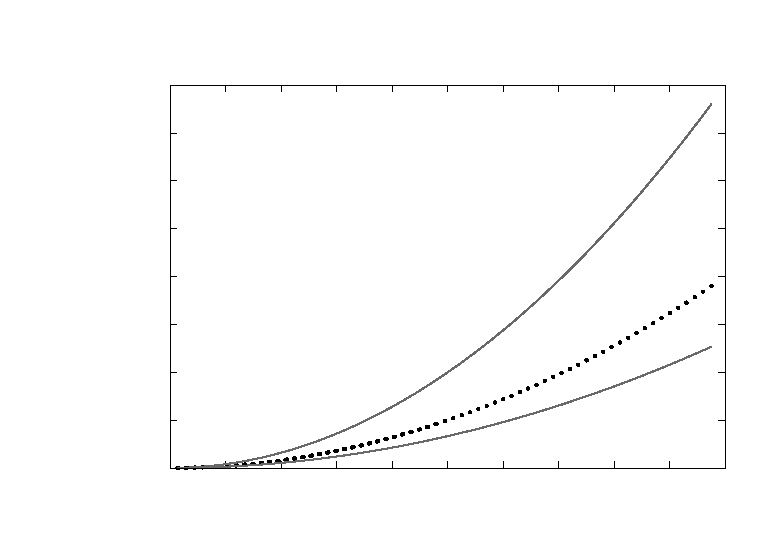
\includegraphics{output_bf}}%
    \gplfronttext
  \end{picture}%
\endgroup

\end{center}

An examination of the code itself explains the empirical results when we observe that there is a doubly-nested for loop that iterates over the input size. 

Therefore, since the brute-force algorithm always runs to completion we conclude that the algorithm is described by

\[
T(n) \in \Theta( n^{2} )
\]

\clearpage
To analyze the divide-and-conquer algorithm, we chose calling the distance method on lines 92 and 99--103 and calculating the distance on lines 150--153 as the basic operations, because these happen most frequently, and are the philosophical heart of this algorithm. There was also the option of choosing the comparison to find the minimum distance (lines 102--103), but compared to finding the distance, it is much less expensive to compare two numbers rather than compute.

An empirical analysis of running the algorithm for multiple values of
$n$ produces the results shown below. The standard function $f(n) = n$ log$(n)$ with constant multipliers, has been added to
illustrate the analysis.

\begin{center}
    % GNUPLOT: LaTeX picture with Postscript
\begingroup
  \makeatletter
  \providecommand\color[2][]{%
    \GenericError{(gnuplot) \space\space\space\@spaces}{%
      Package color not loaded in conjunction with
      terminal option `colourtext'%
    }{See the gnuplot documentation for explanation.%
    }{Either use 'blacktext' in gnuplot or load the package
      color.sty in LaTeX.}%
    \renewcommand\color[2][]{}%
  }%
  \providecommand\includegraphics[2][]{%
    \GenericError{(gnuplot) \space\space\space\@spaces}{%
      Package graphicx or graphics not loaded%
    }{See the gnuplot documentation for explanation.%
    }{The gnuplot epslatex terminal needs graphicx.sty or graphics.sty.}%
    \renewcommand\includegraphics[2][]{}%
  }%
  \providecommand\rotatebox[2]{#2}%
  \@ifundefined{ifGPcolor}{%
    \newif\ifGPcolor
    \GPcolorfalse
  }{}%
  \@ifundefined{ifGPblacktext}{%
    \newif\ifGPblacktext
    \GPblacktexttrue
  }{}%
  % define a \g@addto@macro without @ in the name:
  \let\gplgaddtomacro\g@addto@macro
  % define empty templates for all commands taking text:
  \gdef\gplbacktext{}%
  \gdef\gplfronttext{}%
  \makeatother
  \ifGPblacktext
    % no textcolor at all
    \def\colorrgb#1{}%
    \def\colorgray#1{}%
  \else
    % gray or color?
    \ifGPcolor
      \def\colorrgb#1{\color[rgb]{#1}}%
      \def\colorgray#1{\color[gray]{#1}}%
      \expandafter\def\csname LTw\endcsname{\color{white}}%
      \expandafter\def\csname LTb\endcsname{\color{black}}%
      \expandafter\def\csname LTa\endcsname{\color{black}}%
      \expandafter\def\csname LT0\endcsname{\color[rgb]{1,0,0}}%
      \expandafter\def\csname LT1\endcsname{\color[rgb]{0,1,0}}%
      \expandafter\def\csname LT2\endcsname{\color[rgb]{0,0,1}}%
      \expandafter\def\csname LT3\endcsname{\color[rgb]{1,0,1}}%
      \expandafter\def\csname LT4\endcsname{\color[rgb]{0,1,1}}%
      \expandafter\def\csname LT5\endcsname{\color[rgb]{1,1,0}}%
      \expandafter\def\csname LT6\endcsname{\color[rgb]{0,0,0}}%
      \expandafter\def\csname LT7\endcsname{\color[rgb]{1,0.3,0}}%
      \expandafter\def\csname LT8\endcsname{\color[rgb]{0.5,0.5,0.5}}%
    \else
      % gray
      \def\colorrgb#1{\color{black}}%
      \def\colorgray#1{\color[gray]{#1}}%
      \expandafter\def\csname LTw\endcsname{\color{white}}%
      \expandafter\def\csname LTb\endcsname{\color{black}}%
      \expandafter\def\csname LTa\endcsname{\color{black}}%
      \expandafter\def\csname LT0\endcsname{\color{black}}%
      \expandafter\def\csname LT1\endcsname{\color{black}}%
      \expandafter\def\csname LT2\endcsname{\color{black}}%
      \expandafter\def\csname LT3\endcsname{\color{black}}%
      \expandafter\def\csname LT4\endcsname{\color{black}}%
      \expandafter\def\csname LT5\endcsname{\color{black}}%
      \expandafter\def\csname LT6\endcsname{\color{black}}%
      \expandafter\def\csname LT7\endcsname{\color{black}}%
      \expandafter\def\csname LT8\endcsname{\color{black}}%
    \fi
  \fi
    \setlength{\unitlength}{0.0500bp}%
    \ifx\gptboxheight\undefined%
      \newlength{\gptboxheight}%
      \newlength{\gptboxwidth}%
      \newsavebox{\gptboxtext}%
    \fi%
    \setlength{\fboxrule}{0.5pt}%
    \setlength{\fboxsep}{1pt}%
\begin{picture}(7200.00,5040.00)%
    \gplgaddtomacro\gplbacktext{%
      \csname LTb\endcsname%
      \put(946,704){\makebox(0,0)[r]{\strut{}$0$}}%
      \put(946,1112){\makebox(0,0)[r]{\strut{}$500$}}%
      \put(946,1521){\makebox(0,0)[r]{\strut{}$1000$}}%
      \put(946,1929){\makebox(0,0)[r]{\strut{}$1500$}}%
      \put(946,2337){\makebox(0,0)[r]{\strut{}$2000$}}%
      \put(946,2746){\makebox(0,0)[r]{\strut{}$2500$}}%
      \put(946,3154){\makebox(0,0)[r]{\strut{}$3000$}}%
      \put(946,3562){\makebox(0,0)[r]{\strut{}$3500$}}%
      \put(946,3971){\makebox(0,0)[r]{\strut{}$4000$}}%
      \put(946,4379){\makebox(0,0)[r]{\strut{}$4500$}}%
      \put(1078,484){\makebox(0,0){\strut{}$0$}}%
      \put(1651,484){\makebox(0,0){\strut{}$200$}}%
      \put(2223,484){\makebox(0,0){\strut{}$400$}}%
      \put(2796,484){\makebox(0,0){\strut{}$600$}}%
      \put(3368,484){\makebox(0,0){\strut{}$800$}}%
      \put(3941,484){\makebox(0,0){\strut{}$1000$}}%
      \put(4513,484){\makebox(0,0){\strut{}$1200$}}%
      \put(5086,484){\makebox(0,0){\strut{}$1400$}}%
      \put(5658,484){\makebox(0,0){\strut{}$1600$}}%
      \put(6231,484){\makebox(0,0){\strut{}$1800$}}%
      \put(6803,484){\makebox(0,0){\strut{}$2000$}}%
      \put(2796,1766){\rotatebox{37}{\makebox(0,0)[l]{\strut{}1/3 nlog(n)}}}%
      \put(2796,875){\rotatebox{12}{\makebox(0,0)[l]{\strut{}1/10 nlog(n)}}}%
    }%
    \gplgaddtomacro\gplfronttext{%
      \csname LTb\endcsname%
      \put(176,2541){\rotatebox{-270}{\makebox(0,0){\strut{}Operation Count}}}%
      \put(3940,154){\makebox(0,0){\strut{}Input Size}}%
      \put(3940,4709){\makebox(0,0){\strut{}Empirical Analysis of Brute Force Closest Pair Problem}}%
    }%
    \gplbacktext
    \put(0,0){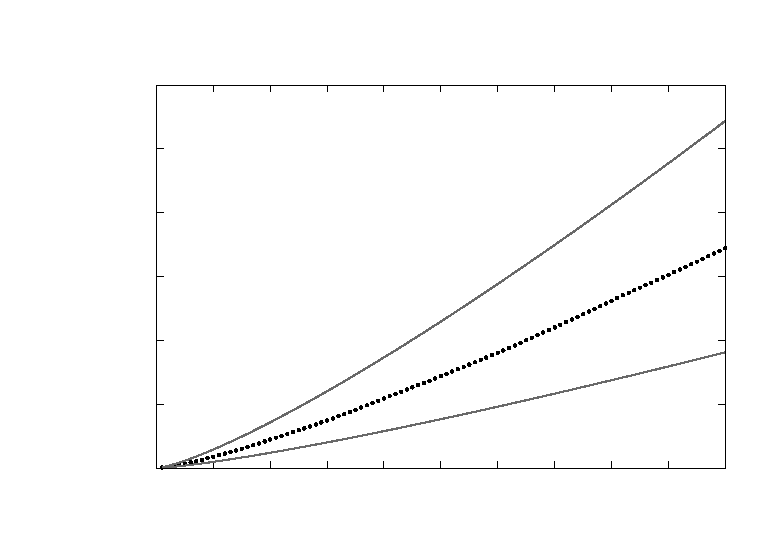
\includegraphics{output_dc}}%
    \gplfronttext
  \end{picture}%
\endgroup

\end{center}

An examination of the code itself explains the empirical results when we observe that this algorithm is recursive, lending us the ability to use the Master Theorem, which is of the form
\begin{center}
	$T(n)=aT(\frac{n}{b}) + f(n)$ where $a \geq 1, b > 1$
\end{center}

Now, this algorithm has two recursive calls, each recursive call operates on half of the input, and $f(n) \in \Theta( n )$ where $f(n)$ is the local work, because both dividing the problem in half and combining the solutions take linear time. Thus, applying the Master Theorem with $a,b,$ and $d$ equal to $2,2$, and $1$ respectively, we get $T(n) \in \Theta(n$ log($n$)).

In addition, the input does not need to be pre-sorted, since using a $O(n $ log$(n)$) efficiency sorting algorithm will not change the asymptotic behavior of this algorithm. 

Therefore, since the divide-and-conquer algorithm always runs to completion we conclude that the algorithm is described by

\begin{center}
$T(n) \in \Theta( n $ log$(n)$)
\end{center}

\end{document}